\documentclass[12pt,a4paper]{scrartcl}		% KOMA-Klassen benutzen!

%\usepackage[ngerman]{babel}			% deutsche Namen/Umlaute
\usepackage[utf8]{inputenc}			% Zeichensatzkodierung
\usepackage{url}
\usepackage{graphicx}
\usepackage[colorlinks=false, pdfborder={0 0 0}]{hyperref}
\usepackage{amsmath}
\usepackage{multicol}

\usepackage{setspace} % Anderthalbfacher Zeilenabstand ist Standard in den meisten Seminararbeiten. Das Paket setspace ermöglicht ein einfaches Umstellen von normalem, anderthalbfachen oder sogar doppeltem Zeilenabstand. 
\usepackage[paper=a4paper,inner=25mm,outer=20mm,top=15mm,bottom=20mm]{geometry} %Das geometry Paket dient zur Einrichtung der Seiten. Hier werden die jeweiligen Seitenränder angegeben. Diese wWerte sollten durch die jeweiligen Vorgaben des Seminarleiters oder Instituts ersetzt werden.
\setlength{\parindent}{1.7em} %Neue Abschnitte werden mit hängendem Einzug gesetzt, parindent definiert. um wie viel der Absat eingerückt wird. Die Einheit em ist abhängig vom verwendeten Zeichensatz und daher absoluten Werten in mm oder cm vorzuziehen. 
\setcounter{secnumdepth}{3} %Bis zu welcher Gliederungsebene nummeriert werden soll gibt dieser Befehl vor. In diesem Falle werden \section, \subsection und \subsubsection nummereiert.
\setcounter{tocdepth}{3} %Bis zu welcher Ebene Einträge ins Inhaltsverzeichnis aufgenommen werden. In diesem Beispiel ebenfalls bis Ebene drei (\subsubsection). Ein durch \paragraph ausgewiesener Abschnitt wird demnach nicht im Inhaltsverzeichnis auftauchen. 

\newcommand{\citeurl}[2]{\url{#1} (#2)}

\begin{document}
\title{HadoopDB}
\subtitle{a major step towards a dead end\\
Thema 5\\Seminar 01912\\ Sommersemester 2011}
\author{Referent: Thomas Koch}
\date{\today}
\maketitle{}

\newpage{}
\tableofcontents{}
\newpage{}

This paper presents and discusses two texts about HadoopDB\cite{journals/pvldb/AbouzeidBARS09} and the Apache Hive\cite{Thusoo_hive-a} project which is used by former.

\section{HadoopDB}

\subsection{Scope and Motivation}

The HadoopDB project aims to combine the scalability advantages of MapReduce with the performance and efficiency advantages of parallel databases. Parallel databases in this context are defined as ``analytical DBMS systems [sic] that deploy on a shared-nothing architecture''. 
Current parallel databases are usually scaled only into the tens of nodes. It may be impossible to scale them into hundreds or thousand nodes like MapReduce for at least three reasons:

\begin{enumerate}
\item Failures become frequent at this scale but the systems don't handle them well.
\item A homogeneous cluster of machines is assumed which is impossible to provide at higher scale.
\item The systems has not yet been tested at this scale.
\end{enumerate}

MapReduce on the other hand is known to scale well into thousands of nodes. However, according to work done by Stonebraker and others, MapReduce would neither be suitable for analytical work\cite{sto08stepback} nor perform well\cite{Pavlo09}.

A further advantage of HadoopDB should be low cost. This could be achieved by building on existing open source solutions: The MapReduce implementation Apache Hadoop, Apache Hive and the RDBMS PostgreSQL. It may however be argued whether these components could be ``used without cost'' as claimed. The production use of software like Hadoop and PostgreSQL still requires highly qualified and payed personal.

\paragraph{Desired Properties}
The following list presents the desired properties of the HadoopDB project together with first comments. It is argued that neither MapReduce nor parallel databases would provide all of these properties.

\begin{itemize}
\item Performance: It is claimed, that performance differences could ``make a big difference in the amount, quality, and depth of analysis a system can do''. Also performance could significantly reduce the cost of an analysis if fewer hardware ressources were used. However Stonebraker and Abadi concluded already in 2007 that the primary factor for costs has shifted from hardware to personal.\cite[2.5 No Knobs]{sto07} It should also be considered that the costs for licenses of proprietary database systems often outrun hardware costs by orders of magnitude. Finally it is not at all certain, that in practice performance differences are a limitation factor for the range of possible computations.

The paper suggests that current practice in analytical systems would be to load data in a specialized database and to make calculations while an operator is waiting for the results. In MapReduce systems however calculations are directly done on the original data and could therefor run continuously during the normal operation of the system. The performance of calculations may therefor not be a practical problem at all.

\item Fault Tolerance:  The probability, that at least one cluster node fails during a computation may be negligible for less then 100 nodes. With growing data size however the cluster needs to grow. Therefor the probability of a single node failure grows as well as the duration of algorithms. This continues until it's not possible anymore to finish calculations without a single node failing.

A system that restarts the whole computation on a single node failure, as typical in RDBMSs, may never be able to complete on large enough data sizes.

\item Ability to run in a heterogeneous environment: Most users of a large cluster would not be able to provide a large number of totally identical computer nodes and to keep there configuration in sync. But even then the performance of components would degrade at different pace and the cluster would become heterogeneous over time. In such an environment work must be distributed dynamically and take node capacity into account. Otherwise the performance could become limited by the slowest nodes.

\item Flexible query interface: The system should support SQL to integrate with existing (business intelligence) tools. Ideally it also supports user defined functions (UDF) and manages their parallel execution.

\end{itemize}
The above list does not include energy efficiency as a desired property although it is one of the most important subjects in recent discussions about data centers.\footnote{see Googles Efficient Data Center Summits \citeurl{http://www.google.com/corporate/datacenter/summit.html}{2011-06-19} and Facebooks open compute project \citeurl{http://opencompute.org}{2011-06-19}} It has also been argued, that standard performance benchmarks should be enhanced to measure the performance relative to energy consumption.\cite{Fanara:2009:SEP:1692899.1692904}

Section 4 describes the parallel databases and MapReduce in further detail. From the desired properties the former would score well on performance and the flexible interface and the later on scalability and the ability to run in a heterogeneous environment. A paper of Stonebraker, Abadi and others\cite{Pavlo09} is cited for the claim of MapReduces lack of performance. This paper is cited over twenty times in the full HadoopDB text and is also the source for the benchmarks later discussed. Other evidence for a lack of performance of MapReduce is not provided.

It is also recognized that MapReduce indeed has a flexible query interface in that it default usage requires the user to provide map and reduce functions. Furthermore the Hive project provides a SQL like interface to Hadoop. Thus although it isn't explicitly said it could be concluded that MapReduce also provides a flexible query interface.

It can be summed up at this point, that MapReduce is excellent in two of four desired properties, provides a third one and only lacks in some degree in performance. Hadoop is still a very young project and will certainly improve its performance in the future. It may be asked, whether a project like HadoopDB is still necessary, if Hadoop itself already provides nearly all desired properties.

It is interesting, how the great benefit of not requiring a schema up-front is turned into a disadvantage against MapReduce:
\begin{quote}
By not requiring the user to first model and
load data before processing, many of the performance enhancing
tools listed above that are used by database systems are not possible.
Traditional business data analytical processing, that have standard
reports and many repeated queries, is particularly, poorly suited for
the one-time query processing model of MapReduce.
\end{quote}
Not requiring to first model and load data provides a lot of flexibility and saves a lot of valuable engineering time. This benefit should be carefully evaluated and not just traded against performance. The quote also reveals another possible strategy to scale analytical processing: Instead of blaming MapReduce for its favor of one-time query processing, the analytical software could be rewritten to not repeat queries. We'll see below that Hive provides facilities to do exactly that by allowing the reuse of SELECT statements.

\subsection{Architecture}
Hive is a tool that provides a SQL interface to MapReduce. It translates SQL queries into apropriate combinations of map and reduce jobs and runs those over tabular data stored in HDFS. HadoopDB extends Hive in that HDFS is replaced by node local relational databases.

\begin{figure}[t]
  \centering
  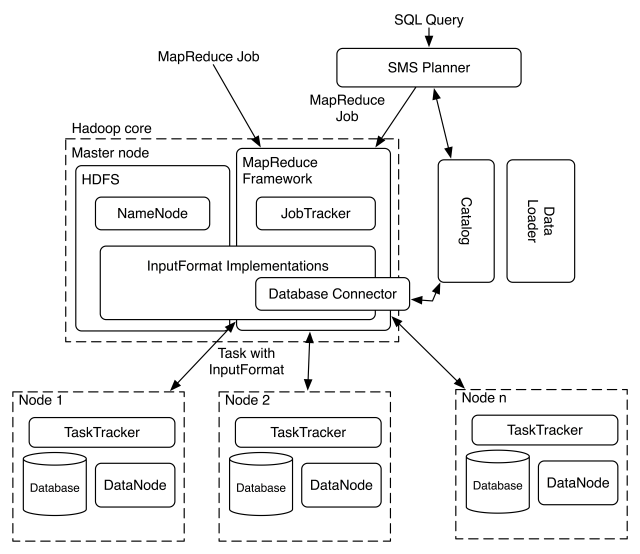
\includegraphics[width=0.7\textwidth]{images/hadoopdb-arch.png}
  \caption{The Architecture of HadoopDB\cite{journals/pvldb/AbouzeidBARS09}}
  \label{fig:hadoopdbarch}
\end{figure}

\paragraph{Data Loader}
HadoopDB comes with two executable java classes and a python script\footnote{\citeurl{http://hadoopdb.sourceforge.net/guide}{2011-06-20}} necessary to partition and load the data into HadoopDB. The data loading is a cumbersome process with several manual steps. Most of the steps must be executed in parallel on all nodes by some means of parallel ssh execution. This leaves a lot of room for failures. It is also necessary to specify the number of nodes in advance. A later change in the number of nodes requires to restart the data load process from scratch. It is also not possible to incrementally add data.

The following list describes the necessary steps to load data into HadoopDB. At each step it is indicated how often the full data set is read (r) and written (w). It is assumed, that the data already exists in tabular format in HDFS and that HDFS is used for this process with a replication factor of 1. This means that in case of a hard drive failure during the import process the process would need to be started again from the beginning. A higher replication factor would lead to even higher read and write numbers in the following list.

\begin{enumerate}
\item Global Hasher: Partition the data set into as many parts as the nodes in the cluster. (2r, 2w + 1 network copy)\footnote{The result of the map phase is written to disk and from there picked up by the reduce phase.}
\item Export the data from HDFS into each nodes local file system. (1r, 1w)\footnote{It is not clear, why this step is necessary. The reduce output from the previous step could have been written directly to the local file systems of the nodes running the reduce jobs.}
\item Local Hasher: Partition the data into smaller chunks. (1r, 1w)
\item Import into local databases. (1r, 1w + secondary indices writes)
\end{enumerate}

We can see, that before any practical work has been done, HadoopDB implies five full table scans and writes. In the same time at least 2.5 map and 2.5 reduce jobs could have completed. If we assume that the results of typical map and reduce jobs are usually much smaller then the input, even more work could have been done. There are indications that it may be possible to optimize the data loading process to lower the number of necessary read and writes. It will be discussed in the benchmark section, why this doesn't seem to be of high priority for the HadoopDB authors.

Neither the HadoopDB paper nor the guide on sourceforge make it totally clear what the purpose of the Local Hasher is. It is suggested that a partitioning in chunks of 1GB is necessary to account for practical limitations of postgreSQL when dealing with larger files.\footnote{``We recommend chunks of 1GB, because typically they can be efficiently processed by a database server.''}

\paragraph{SQL to MapReduce to SQL (SMS) Planner}
The heart of HadoopDB is the SMS planner. Hive translates SQL like queries into directed-acyclic graphs (DAGs) of ``relational operators (such as filter, select (project), join, aggregation)''. These operator DAGs (the query plan) are then translated to a collection of Map and Reduce jobs and sent to Hadoop for execution. In general before each JOIN or GROUP BY operation data must be shared between nodes. 

The HadoopDB project hooks into Hive just before the operations DAG gets sent to Hadoop MapReduce.(Figure~\ref{fig:hadoopdbarch}) The planner walks up the DAG and transforms ``all operators until the first repartitioning operator with a partitioning key different from the database's key'' back into SQL queries for the underlying relational database. 

For those SQL queries where HadoopDB can push parts of the query into the database one could expect a performance gain from secondary indices and query optimization. For other SQL queries one should expect the same performance as with plain Hive. In contrast to Hive HadoopDB can and does take advantage of tables that are repartitioned by a join key and pushes joins over these keys in the database layer.

\paragraph{Auxiliary Components}
HadoopDB includes code to connect to the local databases and a catalog that stores database connection parameters and metadata ``such as data sets contained in the cluster, replica locations, and data partitioning properties''. The catalog must also be generated manually from two input files which adds to the work necessary to setup the data.

\subsection{Benchmarks}

Five different tasks are provided to benchmark two parallel databases (Vertica, DBMS-X), Hadoop and HadoopDB on three different number of nodes (10, 50, 100). The tasks are executed in two different ways. The first round assumes no node failures. Thus the replication factor of HDFS respectively the number of replicas in HadoopDB is set to 1 and the task run is not counted in case of a node failure. In a second round node failures are also taken into account and the replication factor is set to 2.

The tasks are borrowed from the already mentioned Stonebraker paper\cite{Pavlo09}. It is therefor necessary to refer to Stonebrakers work for their description at some points.

\subsubsection{Data Sets}

\begin{figure}
  \centering
  \begin{multicols}{2}
\begin{verbatim}
CREATE TABLE Documents (
  url VARCHAR(100) PRIMARY KEY,
  contents TEXT 
);

CREATE TABLE Rankings (
  pageURL VARCHAR(100) PRIMARY KEY,
  pageRank INT,
  avgDuration INT 
);
\end{verbatim}    

\begin{verbatim}
CREATE TABLE UserVisits (
  sourceIP VARCHAR(16),
  destURL VARCHAR(100),
  visitDate DATE,
  adRevenue FLOAT,
  userAgent VARCHAR(64),
  countryCode VARCHAR(3),
  languageCode VARCHAR(6),
  searchWord VARCHAR(32),
  duration INT 
);
\end{verbatim}
  \end{multicols}
  \caption{Tables used for the analytical benchmark tasks.}
  \label{fig:tableschemas}
\end{figure}

The first task (Grep) uses a simple schema of a 10 bytes key and a random 90 bytes value field. The next three analytical tasks work on a more elaborate schema of three tables. (Figure~\ref{fig:tableschemas}) This schema was originally developed by Stonebraker and others to argue that parallel databases could also be used in areas where MapReduce recently became popular.\cite[1.]{Pavlo09} The Documents table should resemble the data ``a web crawler might find'' while the UserVisits table should ``model log files of HTTP server traffic''. The Rankings table is not further described.\cite[4.3]{Pavlo09}

It seems that Stonebraker has a very naive idea of the inner workings of a typical web crawler and the information typically logged by a HTTP server. The BigTable paper from 2006 explains, that Google stores multiple versions of crawled data while a garbage collector automatically removes the oldest versions.\cite{Chang:2006:BDS:1267308.1267323} This requirement alone would be very complicate to model on top of a relational data store. Furthermore a web crawler would certainly store a lot more data, for example the HTTP headers sent and received, which may be several pairs due to HTTP redirects or a history when the page was last loaded successfully along with the last failed loading attempts and the reasons for those failures. Subsequental processes enrich the data for example with data extracted from HTML or the HTTP headers and with a list of web sites pointing to this site (inlinks) together with the anchor text and the page rank of the inlinks. The pageRank column from the Rankings table would surely be inlined into the Documents table.

The UserVisits table is likely unrealistic. A HTTP server usually has no knowledge of any adRevenue related to a web site just served, nor is anything known about a searchWord. Web sites that highlight search words used previously in a search engine to find that page do so by parsing the HTTP referrer header. A HTTP server is usually not capable to extract this information. The same is valid for the HTTP accept language header which provides a languageCode. A countryCode can usually only be obtained by looking up the users IP address in a so called geoIP database.

The most important flaw in the data sets however is the assumption of a separated, off line data analytics setting. Todays search engines need to reflect changes in crawled pages as soon as possible. It is therefor typical to run the whole process of crawling, processing and indexing on the same database continuously and in parallel.\cite{Peng:2010:LIP:1924943.1924961}

It is understandable that Abadi choose to reuse the benchmarks to enable comparison. However he wants to demonstrate the applicability of HadoopDB ``for Analytical Workloads''. One should expect benchmarks that use schemes related to financial, customer, production or marketing data.

\paragraph{Data Loading}
It has already be described how complicate the data loading procedure is. The benchmark measured a duration of over 8.3 hours for the whole process. Since the process is not (yet) automatized and may even need to be restarted from scratch in case of failures, it can in practice take two working days. The HadoopDB authors however do not consider this to be a problem\cite[6.3]{journals/pvldb/AbouzeidBARS09}:

\begin{quote}
While HadoopDB’s load time is about 10 times longer than
Hadoop’s, this cost is amortized across the higher performance of
all queries that process this data. For certain tasks, such as the Join
task, the factor of 10 load cost is immediately translated into a
factor of 10 performance benefit.
\end{quote}

This statement however ignores that data is often already stored on Hadoop in the first place and that Hadoop wouldn't require a load phase at all. Instead Hadoop could run analytical tasks incrementally or nightly and provide updated results while HadoopDB still struggles to load the data.

\subsubsection{Grep Task}
The Grep Task executes a very simple statement over the already described key value data set:
\begin{verbatim}
SELECT * FROM Data WHERE field LIKE '%XYZ%';
\end{verbatim}
Hadoop performs in the same area as HadoopDB and the parallel databases require less then half the time. It is argued that this difference in performance in such a simple query is mainly due to the use of data compression by the parallel databases and therefor faster scan times. Although Hadoop supports compression and could therefor share the same benefits, it isn't used. An explanation is found in the Stonebraker paper. They did some experiments with and without compression and in their experience Hadoop did not benefit but even get slower.

However it seems that there could be mistakes in their usage of Hadoop. Instead of using the Hadoop SequenceFile format to write compressed data, they split the original files in smaller files and used a separate gzip tool to compress them. There is no explanation why they did the splitting nor do they provide the compression level used with gzip. It is very likely that the raise in the number of files caused by the splits led to a higher number of necessary disc seeks.

They also tried record-level compression. This is however pointless since the values in the Grep Task have only a length of 90 bytes and may even get larger from the compression header.

\subsubsection{Selection Task}
The selection task executes the following query:
\begin{verbatim}
SELECT pageUrl, pageRank FROM Rankings WHERE pageRank > 10;
\end{verbatim}

The description and result diagram for this task is a bit confusing, because the text says that HadoopDB would outperform Hadoop while the diagram on first sight reports comparable execution times for both. The solution is that there is a second bar for HadoopDB reporting the duration for a data repartitioning that has been optimized for this task.

It is questionable whether the long and complicate data loading is still tolerable, if it even has to be optimized for different queries. One would expect that the upfront investment of data modeling and loading would be rewarded by a great variety of possible queries that could be executed afterward with high performance.

\subsubsection{Aggregation Tasks}
These two tasks differ only in their grouping on either the full sourceIP or only a prefix of it.

\begin{verbatim}
SELECT SUBSTR(sourceIP, 1, 7), SUM(adRevenue) FROM UserVisits 
GROUP BY SUBSTR(sourceIP, 1, 7);
\end{verbatim}
\begin{verbatim}
SELECT sourceIP, SUM(adRevenue) FROM UserVisits 
GROUP BY sourceIP;
\end{verbatim}

Hadoop and HadoopDB differ only in around 20\% of their execution time while the parallel databases are again significantly faster. It is once again argued that this would be mainly caused by compression and therefor the same arguments apply as with the Grep Task.

Furthermore this tasks points out the advantage of a high level access language. Hive (and thereby HadoopDB) benefited from automatically selecting hash- or sort-based aggregation depending on the number of groups per rows. A hand coded MapReduce job will most likely have one of these strategies hand coded.

\subsubsection{Join Task}
The join task needed to be hand coded for HadoopDB too, due to implementation bugs. The equivalent SQL is:
\begin{verbatim}
SELECT sourceIP, COUNT(pageRank), SUM(pageRank),
SUM(adRevenue) FROM Rankings AS R, UserVisits AS UV
WHERE R.pageURL = UV.destURL AND
UV.visitDate BETWEEN '2000-01-15' AND '2000-01-22'
GROUP BY UV.sourceIP;
\end{verbatim}

In this task HadoopDB performs ten times faster then Hadoop but still significantly slower then the parallel databases. The databases (including HadoopDB) are said to benefit from a secondary index on visitDate, the selection predicate. There are however at least three questions to be asked about this task.

First, why would anybody want to run this query only for the specified weeks and not for all weeks? If this query would be run for all weeks then the databases would also need to scan all data and maybe approach the duration of Hadoop. Hadoop on the other hand would typically run a nightly run over its data to produce small daily statistics which in turn could be easily imported into a traditional relational database.

Second, as already noted the UserVisits table hardly resembles a typical server log. A typical server log would be ordered by visitDate. If the visitDate would be the primary key, then Hadoop should be able to execute the query much faster.

Third, since the UserVisits table already contains data from other sources (adRevenue, countryCode, languageCode, searchWord), why isn't there also a column for page rank? This would of course duplicate data and break traditional database design but better match real world scenarios. In this case the join wouldn't be needed and the task would be mostly the same as the selection task already discussed.

\subsubsection{UDF Aggregation Task}
This task represents the prime example of MapReduce. The data set consists of a large corpus of HTML documents. Those are parsed and the occurrence frequency of every url gets counted. Not only was it difficult to implement this task with the parallel databases, they also performed significantly worse then Hadoop. HadoopDB wasn't used with it's SQL layer but also queried by MapReduce. 

\subsubsection{Fault tolerance and heterogeneous environment}
All discussed tasks so far have been executed optimistically without any precautions for single node failures. To test the different performance of the systems in the presence of failures and in a heterogeneous environment the aggregation task with grouping on the prefixed sourceIP has been repeated. This time the replication factor was set to 2 and for the fault tolerance test one random node was killed when half of the query was executed. The heterogeneous environment was tested in another round by slowing done one node by running an I/O intensive background job and frequent clears of the OS caches.

The performance loss is reported relatively to the normal performance. Vertica suffers a dramatic slowdown of over 100\% in both cases since it restarts queries from the beginning on failure and does not move straggling tasks to other nodes. HadoopDB and Hadoop both profit from Hadoops inherent design for frequent failures. First Hadoop does not restart the whole query from scratch when one node fails but only that part of the query that the failed node performed. Second Hadoop runs second instances of straggling tasks on already finished nodes. This is called speculative execution. The later started tasks may finish earlier then tasks that run on faulty nodes with degraded performance.

HadoopDB slightly outperforms Hadoop in the case of failing nodes. Hadoop is slowed down in this case because it is eager to create additional copies of the replicated data to provide the replication factor again as soon as possible. HadoopDB on the other hand does not copy data and would therefor suffer a data loss in case that two nodes containing the same data would fail.

\subsection{Summary}
The HadoopDB authors conclude that HadoopDB would outperform Hadoop in all but the last tasks and that it would therefor be a useful tool for large scale analytics workloads.

 The comments and discussions in the preceding subsections however challenge this conclusion. The long time to load data may be a problem. Some of the provided benchmarks are rather unrealistic. The number of nodes tested is still a lower limit for typical MapReduce installations. The usage of Hadoop may not have been optimal as seen in the discussion about compression. An experienced Hadoop engineer may be able to achieve better results with the given tasks. The fault tolerance of HadoopDB lacks the self healing mechanism of HDFS. And HadoopDB is designed to be a read only database parallel to the production databases. This seems to be a contradiction to the authors own remark that it would be ``a requirement to perform data analysis inside of the DBMS, rather than pushing data to external systems for analysis''.

\section{Hive}

Hive has been developed by facebook as a petabyte scale data warehouse on top of Hadoop.\cite{Thusoo_hive-a} A typical use case for hive is to store and analyze incrementally (daily) inserted log data. It provides user interfaces and APIs that allow the submission of queries in a SQL like language called HiveQL. The application then parses the queries to a directed-acyclic graph (DAG) of Map Reduce jobs and executes them using Hadoop.

Data in Hive is stored in tables, which can be partitioned by multiple levels of attributes. Inside a table or a partition data can be further split in so called buckets. The target bucket is choosen by a hash function over a column modulo the desired number of buckets.\footnote{\url{http://wiki.apache.org/hadoop/Hive/LanguageManual/DDL/BucketedTables}} Tables and partitions are represented inside the Hadoop file system as regular directories while buckets are files either in the table directory if there are no partitions or in the last partition directory.

The following is a path of a bucket in the table ``daily\_status'' with partitions on the columns ``ds'' and ``ctry''. The hive workspace is in the ``wh'' directory:

\begin{displaymath}
  /wh/\underbrace{daily\_status}_{\text{table name}}/\underbrace{ds=20090101/ctry=US}_{\text{nested partitions}}/\underbrace{0001}_{\text{bucket}}
\end{displaymath}

Buckets are useful to prototype and test queries on a sample of the full data. Hive provides a SAMPLE clause that lets the user specify the number of buckets that should be used for the query. Although no reference has been found for this thesis, buckets may also be useful to distribute the write and read load to multiple HDFS data nodes.

Hive can not modify already stored data. This was a design decision to avoid complexity overhead. Thus there are no UPDATE or DELETE statements in HiveQL.\cite{hive-icde2010} Regular INSERTs can only write to new tables or new partitions inside a table. Otherwise a INSERT OVERWRITE must be used that will overwrite already existing data. A typical use case adds data to hive once a day and starts a new partition for the current date. Thus there is no practical limitation.

Besides primitive scalar types, hive also provides nestable collections like arrays and maps. Additional types can be programmed by the user.

One component important for the understanding of Hive is the Hive-Metastore. It contains table schemes and should in the future also contain data distribution statistics. The former is needed for data exploration and query parsing. The latter could be used for query optimization.

For extensibility hive provides the ability for user defined (aggregation) functions. One example provided is a Python function used to extract memes from status updates.

A noteworthy optimization is the ability to use a SELECT statement as input for multiple INSERT statements. This allows to minimize the number of table scans.

\begin{verbatim}
FROM (SELECT ...) subq1
INSERT TABLE a SELECT subq1.xy, subq1.xz
INSERT TABLE b SELECT subq1.ab, subq1.xy
\end{verbatim}

\newpage{}


















\section{NoSQL and the end of an architectural era}
In 2007 a paper with the provoking title ``The end of an architectural era:(it's time for a complete rewrite)''\cite{sto07} claimed that the time for traditional relational database management systems would be over. Current RDBMSs have their roots in over thirty years old legacy code lines. They are build on assumptions, requirements and hardware constraints that no longer hold true today and should therefor be replaced by a variety of specialized engines.

The change in Hardware is obvious. Main memory (RAM) on servers, CPU speed, number of CPUs and storage size have all increased by several orders of magnitude while at the same time hardware price decreased. In former times it was feasible to pay high salaries for specialized staff to administrate and optimize hardware. Today it is a decent decision to buy more hardware and spare costly developer time.

At the time systems like SQL Server, DB2 or Oracle were architected, they targeted the only then existing database market which back then was business data processing. Today several new markets exists:

\begin{itemize}
\item Text (search engines, translations, groupware)
\item Data Warehouses
\item Stream Processing (social networks, news sites, real time communication)
\item Scientific and intelligence databases (semantic data)
\end{itemize}

For all this use cases, specialized systems can outperform RDBMSs by a factor of 10.\cite{conf/cidr/StonebrakerBCCGHHLRZ07}. Stonebrakers findings and conclusions correspond with the views of many proponents of the so called ``NoSQL'' movement. His text from 2007 has therefor been proposed as an introductory reading for an international nosqlsummer in 2010.\footnote{\url{http://nosqlsummer.org/papers} The author was the organizer of the nosqlsummer meetings at lake Constance.} 

Although Stonebraker and his co authors (one of them is Daniel J. Abadi, the main author of the HadoopDB paper) make a strong points against RDBMSs and for alternative systems, the next section will discuss how they oppose MapReduce in favor of parallel databases and by doing so ignore their own arguments made against relational systems.

\section{The MapReduce vs. parallel databases debate}
In an online article from January 2008, published on the website of the database company Vertica Systems\footnote
{According to Wikipedia Stonebraker is co-founder of Vertica Systems, which has recently (march 2011) been acquired by HP. Footnote 9 in \cite{journals/pvldb/AbouzeidBARS09} discloses that also Daniel Abadi has a small financial stake in the company.},
Stonebraker heavily criticizes MapReduce.\cite{sto08stepback} The article has been commented (in comments on the same page or in blog posts\cite{Chu-Carrol08hammers}) as being inaccurate or missing the point. The main inaccuracy comes from judging MapReduce in areas which it has not been designed for especially judging it as a DBMS, which it isn't.

Since 2008 MapReduce and its supporting tools have made a lot of progress. Therefor it makes sense to revisit some of the arguments and consider recent developments.

\subsection{Understanding of the term MapReduce}
As Stonebraker rightly points out, MapReduce is not novel. In its core it's just the concept of using a map and a reduce function and in this a basic concept of functional programming. MapReduce can work on different underlying data stores: the Google File System (GFS), Hadoop Distributed File System (HDFS), databases like HBase, Cassandra, Riak, MongoDB and others. These are all systems for large data sets. But MapReduce is also a main building in CouchDB which uses views and B-Trees and targets server installations as well as mobile devices.

In the discussed papers the term MapReduce however is used to describe the combination of a scalable, fault tolerant file system (GFS or HDFS) together with a batch processing execution framework (Hadoop or Google MapReduce).
This inaccurate term usage may contribute to some of the misunderstandings discussed below. This text will however adapt to this nomenclature for the sake of readability.

\subsection{Rebuttal of MapReduce criticism}
\paragraph{Lack of schemes}
MapReduce has no support of schemes since it does not aim to be a database. However the object serialization projects avro, protocol buffers and thrift provide facilities to define schemes in one central place or together with the data and use them from most popular programming languages.\footnote{avro: \url{http://avro.apache.org/}, protocol buffers: \url{http://code.google.com/p/protobuf}, thrift: \url{http://thrift.apache.org}}
Furthermore the HCatalog project\footnote{\url{http://developer.yahoo.com/blogs/hadoop/posts/2011/04/hcatalog-tables-and-metadata-for-hadoop}} has recently been started by the Apache projects Hive and Pig to provide an independent and reusable schema store for data stored in HDFS.

\paragraph{Lack of high level access languages}

Since MapReduce is not a database but a platform it is even possible to implement applications on top of it which would be impossible to model with SQL like machine learning. The Mahout project\footnote{\url{http://mahout.apache.org}} is exactly that.\footnote{some pointers taken from: \url{http://www.hpts.ws/session10/shekita.txt}}

\paragraph{Missing features}
While it may not be fair to compare the tool set of decades of relational database development with those of the young MapReduce world, there is still already quite something to mention for the categories questioned:

\begin{itemize}
\item Bulk loader: Sqoop\footnote{\url{https://github.com/cloudera/sqoop}} is developed by Cloudera to transfer data between Hadoop, relational databases and other means. Besides that there are multiple projects to continuously import stream data into Hadoop: Flume, Scribe and Chukwa\footnote{\url{http://nosql.mypopescu.com/post/820711193/how-does-flume-and-scribe-compare}}.
\item Indexing: The Belgian CMS company Outerthought is pioneering to build its newest CMS on top of HBase and therefor also Hadoop. For its content repository it evaluated different scalable indexing solutions to provide secondary indexes into HBase.\footnote{\url{http://www.lilyproject.org/lily/about/technology.html}} Outerthought has been included by Gartner in "Cool Vendors in Content Management 2010" list.\footnote{\url{http://outerthought.org/blog/373-ot.html}}
\item Updates: MapReduce or better said the Google File System respectively HDFS have been developed for big files that are written once and never changed. On top of that Googles BigTable or Apache HBase provide databases for random access and updates to small data items.
\item Transactions: When Googles BigTable database was implemented, transactions were left out initially. Later on it was observed, that there was actually no real need to support them, because most applications require only row level isolation.\cite[p. 12]{Chang:2006:BDS:1267308.1267323} The developers of the web service streamy.com give a description how they started development with a normalized scheme on a RDBMS and had to denormalize there scheme step by step to scale the service. In the end they gave up on their RDBMS altogether and used HBase instead.\cite[p. 431-435]{White201010}
\item Integrity constraints: As with transactions one can argue that most use cases for MapReduce don't have the need for integrity constraints. Data that is handled by MapReduce is often collected from unreliable or unstructured sources like web pages, log files or sensors. It is desirable to also save corrupted data, like invalid HTML or out of scale measured data. This data can afterward be simply ignored by MapReduce jobs but is still available for further analysis. A search engine could for example reduce the ranking of domains with many invalid HTML pages or in a sensor network one could identify sensors which often produce erroneous values. So in the world of MapReduce integrity is handled at read time, not at write time. Different MapReduce jobs may have different opinions about which data they consider worth of further examination.
\item Referential integrity: See the argument on transactions. When the scheme is denormalized there is no need for referential integrity. Furthermore with data at scale one may need to give up on perfect data. Web links may point to nonexistent pages, Users may have deleted their accounts, changed their name or email address.
\item Views: I'm not aware of anything similar in MapReduce related technology nor have I ever read a complaint about its absence. But as we've seen above, tools on top of MapReduce get developed when needs for them occur.
\end{itemize}
Stonebraker also criticizes an absence of integration with DBMS tools. At least for Business Intelligence this may not be the case anymore since Pentaho announced Hadoop support in may 2010.\footnote{\url{http://www.pentaho.com/news/releases/20100519_pentaho_harnesses_apache_hadoop_to_deliver_big_data_analytics.php}}

\section{Discussion of MapReduce vs. parallel databases benchmarks}
The previous section discussed the misconception about MapReduce being a database. In line with this misconception, Stonebraker, Abadi et al. moved on to directly compare performance between MapReduce and two RDBMSs.\cite{Pavlo09} This section discusses some of the flaws of this work.
The benchmarks were made on a cluster of at maximum 100 machines. This decision is justified by the ``superior efficiency of modern DBMSs'' that would not require more hardware to work on petabyte scale. This argument will be revisited in this section. 
Stonebraker also questions the necessity for such large data sets at all:
\begin{quote}
  Since few data sets in the world even approach a petabyte in size, it is not at all clear how many MR users really need 1.000 nodes.
\end{quote}
This proposition sounds a lot like the famous (mis)quotes ``I think there is a world market for maybe five computers'' and ``640K ought to be enough for anybody''. While it may not be desirable from an energy efficiency or data privacy point of view to have many petabyte clusters, it only needs a little imagination to come up with many valid use cases. Millions of smart phones with cameras produce an immense amount of pictures and videos. Modern cars have sensors and computers build in whose data could (or is?) used to improve the next generation of cars. Science analyzes large data sets in genetics or high energy physics. The Global Biodiversity Information Facility is currently evaluating Hadoop.

\paragraph{Fault Tolerance}
The probability, that at least one cluster node fails during a computation may be negligible for less then 100 nodes. With growing data size the cluster needs to grow. The probability of a single node failure during a fixed time span and the duration of any meaningful algorithm grow faster then linear until it's not possible anymore to finish calculations without a single node failing.

A system that restarts the whole computation on a single node failure, as typical in RDBMSs, may never be able to complete on large enough data sizes.
By limiting the benchmark to a cluster of 100 nodes this problem is practically avoided. Abadi discusses the problem in the HadoopDB work.\cite{journals/pvldb/AbouzeidBARS09}. Still there's no automated failure recovery build into HadoopDB.

\paragraph{Data Loading}
The discussed benchmarks all create a setup in which data is prepared and loaded into a data analytics cluster just for the purpose of the analysis. It is assumed that the data is imported from some other data store that is responsible for reliable long term storage and backup.
This however is not the typical use case of GFS or HDFS. These file systems are used to collect the raw incoming data from crawlers, sensors, log files or user actions. Instead of moving this data to a separate analytic cluster, MapReduce works directly on the original data, perhaps storing the computed data to a separate data store.
The validity of the given benchmarks is therefor highly questionable. A realistic benchmark would need to consider the necessity for reliable storage and parallel writes. A separate ``data loading phase'' however may not be practical in real world scenarios.

\paragraph{Problem Space}
One of the benchmarks, the ``Selection Task'' works on input that already combines a url with its page rank. This may serve as an indicator for the complete misunderstanding of the different problem space of MapReduce opposed to that of RDBMSs. The original MapReduce paper explicitly names the ``Reverse Web-Link Graph'' as an example task for MapReduce. The output of this task is the input to calculate page rank. This algorithm is one of the model use cases for MapReduce.

The benchmark however assumes the page rank as a given input data for a task that is indeed a proper use case for a RDBMS and not for MapReduce. MapReduce users usually do not deny the usefulness of RDBMSs in their appropriate problem space. Facebook for example has been reported to use Oracle and MySQL to analyze data that has been prepared by Hadoop. (Figure~\ref{fig:facebookdatawarehouse})

\begin{figure}[t]
  \centering
  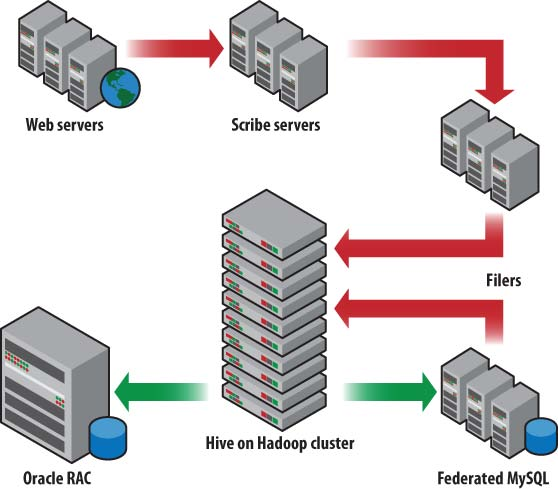
\includegraphics[width=0.7\textwidth]{images/rdms_as_frontend.jpg}
  \caption{Data warehouse architecture at Facebook\cite[p. 508]{White201010}}
  \label{fig:facebookdatawarehouse}
\end{figure}

There are more details to discuss in Stonebrakers benchmarks but this is left to a separate work. Other discussion points are explored in the below sections about HadoopDB.














\subsection{Benchmarks}
The HadoopDB paper uses the same benchmarks as used in Stonebrakers comparison paper. These are
\begin{itemize}

\item Aggregation Task
  \begin{enumerate}
  \item Smaller query:

  \end{enumerate}
  \item Join Task:
An additional reduce job calculates the average pageRank and total adRevenue for each sourceIP. The SQL query for the relational databases directly calculates the average in the above select, stores the result in a temporary table and use a second select to retrieve the row with the highest total revenue.
  \item UDF task: Calculate the inlink count for a dataset of (page url, page html).
\end{itemize}
In most tasks HadoopDB performes in the same range as Hadoop in comparission to the parallel database systems. Hadoop is considerably faster then all other systems in the UDF task, which is also a very typical use case of MapReduce.

Only in the join task HadoopDB is faster by an order of magnitude. It is however not likely, that Hadoop would ever encounter input data in such a strange format as presented in the benchmark. The benchmark pretends two tables for this task.

The first one resembles the access log of a web server with the fields sourceIP, destURL, visitDate, adRevenue, userAgent, countryCode, languageCode, searchWord and duration. 
The selection task diagram shows two different bars for HadoopDB. Without optimization, HadoopDB performed equally slow as Hadoop. Only by optimizing the data partitioning for this specific benchmark could HadoopDB outperform Hadoop by a factor of 2 to 4.

\subsection{Practical evaluation}

An important indicator for the evaluation of computer technology is its impact on the internet. From this perspective, HadoopDB seems to have failed. Google reports\footnote{as of April 7th} less then ten independent mentions of HadoopDB not counting the HadoopDB authors own publications.

Since HadoopDB uses PostgreSQL and provides a solution to cluster this DBMS, one should expect some interest from the PostgreSQL community. There are however only a total of 15 mails in the projects list archive mentioning HadoopDB from which only 4 are from last year.\footnote{as of April 8th \url{http://search.postgresql.org/search?m=1}}

The public subversion repository of HadoopDB on SourceForge has only 22 revisions.\footnote{as of June 14th \url{http://hadoopdb.svn.sourceforge.net/viewvc/hadoopdb}}

Although Hadoop is one of the most discussed award winning free software projects right now, HadoopDB did not manage to profit from this and raise any significant interest at all outside of academic circles. This may be one indicator for the correctness of critiques presented in this paper.

An additional critique from a practical perspective may be the combination of two highly complicate systems, Hadoop and PostgreSQL, that both require advanced skills from the administrator. It is hard enough to find personal that can administrate one of these systems. It may be practically impossible to find personal competent in both. Both systems come with their own complexities that add up for little or no benefit.

As already mentioned, Stonebraker already concluded that new databases must be easy to use because hardware is cheaper then personal. The HadoopDB guide however expects sophisticated manual work:\footnote{\url{http://hadoopdb.sourceforge.net/guide}}
\begin{quote}
"a careful analysis of data and expected queries results in a significant performance boost at the expense of a longer loading. Two important things to consider are data partitioning and DB tuning (e.g. creating indices). Again, details of those techniques are covered in textbooks. For some queries, hash-partitioning and clustered indices improve HadoopDB's performance 10 times"  
\end{quote}



\newpage{}
% http://liinwww.ira.uka.de/bibliography/index.html
% http://de.wikipedia.org/wiki/BibTeX#Bibliographiedatenbanken
\bibliography{references}{}
\bibliographystyle{alphadin}
\end{document}

% LocalWords:  RDBMSs HadoopDB CPUs Stonebrakers nosqlsummer Stonebraker Abadi
% LocalWords:  Vertica Jagl Cloudbase Gartner streamy et al indices
% Local Variables:
% ispell-dictionary: "american"
% eval: (flyspell-mode 1)
% End:
